%
\section{SiCP2, chaîne de pendules couplés}
%
SiCP2 est un simulateur de chaîne de pendule. Un moteur sinusoïdale, carré, ou impulsionnel permet de créer une excitation de l'extrémité de la chaîne. Les conditions aux limites peuvent être périodiques, libres ou fixes. La dissipation peut être uniforme ou simuler une extrémité absorbante.
%
\begin{center}
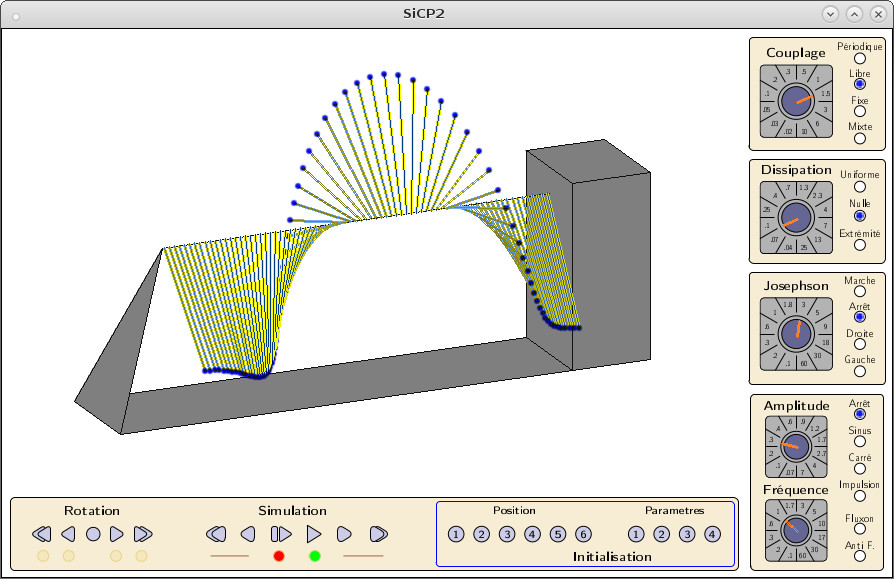
\includegraphics[scale=0.41]{./illustration/SiCP2}
\end{center}
%
Le programme simule l'équation de sine-gordon. Le contrôle du courant josephson permet d'observer la dynamique des solitons.
%
%%%%%%%%%%%%%%%%%%%%%%%%%%%%%%%%%%%%%%%%%%%%%%%%%%%%%%%%%%%%%%%%%%%%%%%%%%%%%%%%%%%%%%%%%%%%%
